
\chapter{Service Work: Jet and \texorpdfstring{\etmiss }{ETmiss} studies (22/11/2017)}

To become more integrated in the Level-1 Trigger, as well as continuing with the JECs and taking on shifts, I've been asked to take over some of the MET studies Batool has previously done. This should all count towards the EPR I need for authorship, and I can check my progress at \url{https://icms.cern.ch/epr/showMine}.

\section{Understanding high-MET events in Zero Bias}

I've been asked to make various plots of events that are firing the \texttt{L1\_MET100} trigger to see if there are obvious issues with hot towers, ECAL spikes, PU mis-estimation, etc. Aaron wrote a macro that can make some plots needed. I modified it to add extra features, extra plots and tidied up some of the code. Then, I bunged everything into a new GitHub repository for version control and safeguarding -- \url{https://github.com/eshwen/High-MET-studies}. One of the revisions of the macro is located here: \href{run:modules/Sec 34 - Service Work - ETmiss studies/figures/MET_studies_v6/doMetStudy.cxx}{doMetStudy.cxx (v6)}.

If I source a CMSSW release that contains the L1Trigger packages (because I need some header files contained within them), i.e., the CMSSW I use for JECs, I can run the macro with

\begin{lstlisting}[belowskip=-0.7cm, language=sh, numbers=none]
root -l -b -q doMETStudy.cxx
\end{lstlisting}

I initially ran on Soolin as that's where the JEC code was. But if I moved the macro to lxplus and set up the environment, I could use the fact that the ntuples were stored locally on AFS to access and run over them much quicker (hence the local file paths in the macro). I also realised I could fill histograms with a weight, rather than just incrementing a bin by 1:

\fcolorbox{red}{pink}{\begin{minipage}{0.9\textwidth}
Using \texttt{h->Fill(quantity, weight)}, I can fill histograms instead of making arrays of different quantities and populating a TGraph. For example, if I wanted to plot the HCAL TP $\ET$ against iPhi, I could do \texttt{h->Fill(hcaliPhi, hcalTPET)} to increment the iPhi bin by the TP $\ET$.
\end{minipage}}

I made various plots of TP $\ET$ against iEta and iPhi for the ECAL, HCAL, towers (sum) and trigger tower (TT) 28. I've made similar plots with $\ET^{\mathrm{T}}$ and \etmiss, as well as plots for individual events to see if the \etmiss came from large spikes or broad PU jets. I included some plots of the "average" TP $\ET$ as well: the total $\ET$ in an iEta/iPhi bin divided by its occupancy, as well as the total $\ET$ divided by the number of events. These could help identify hot towers, inhomogeneous responses or calibrations, etc. Some of the plots are below, the rest are located in \textbf{modules/Sec 34 - Service Work - ETmiss studies/figures/}.

\begin{figure}[htbp]
\centering
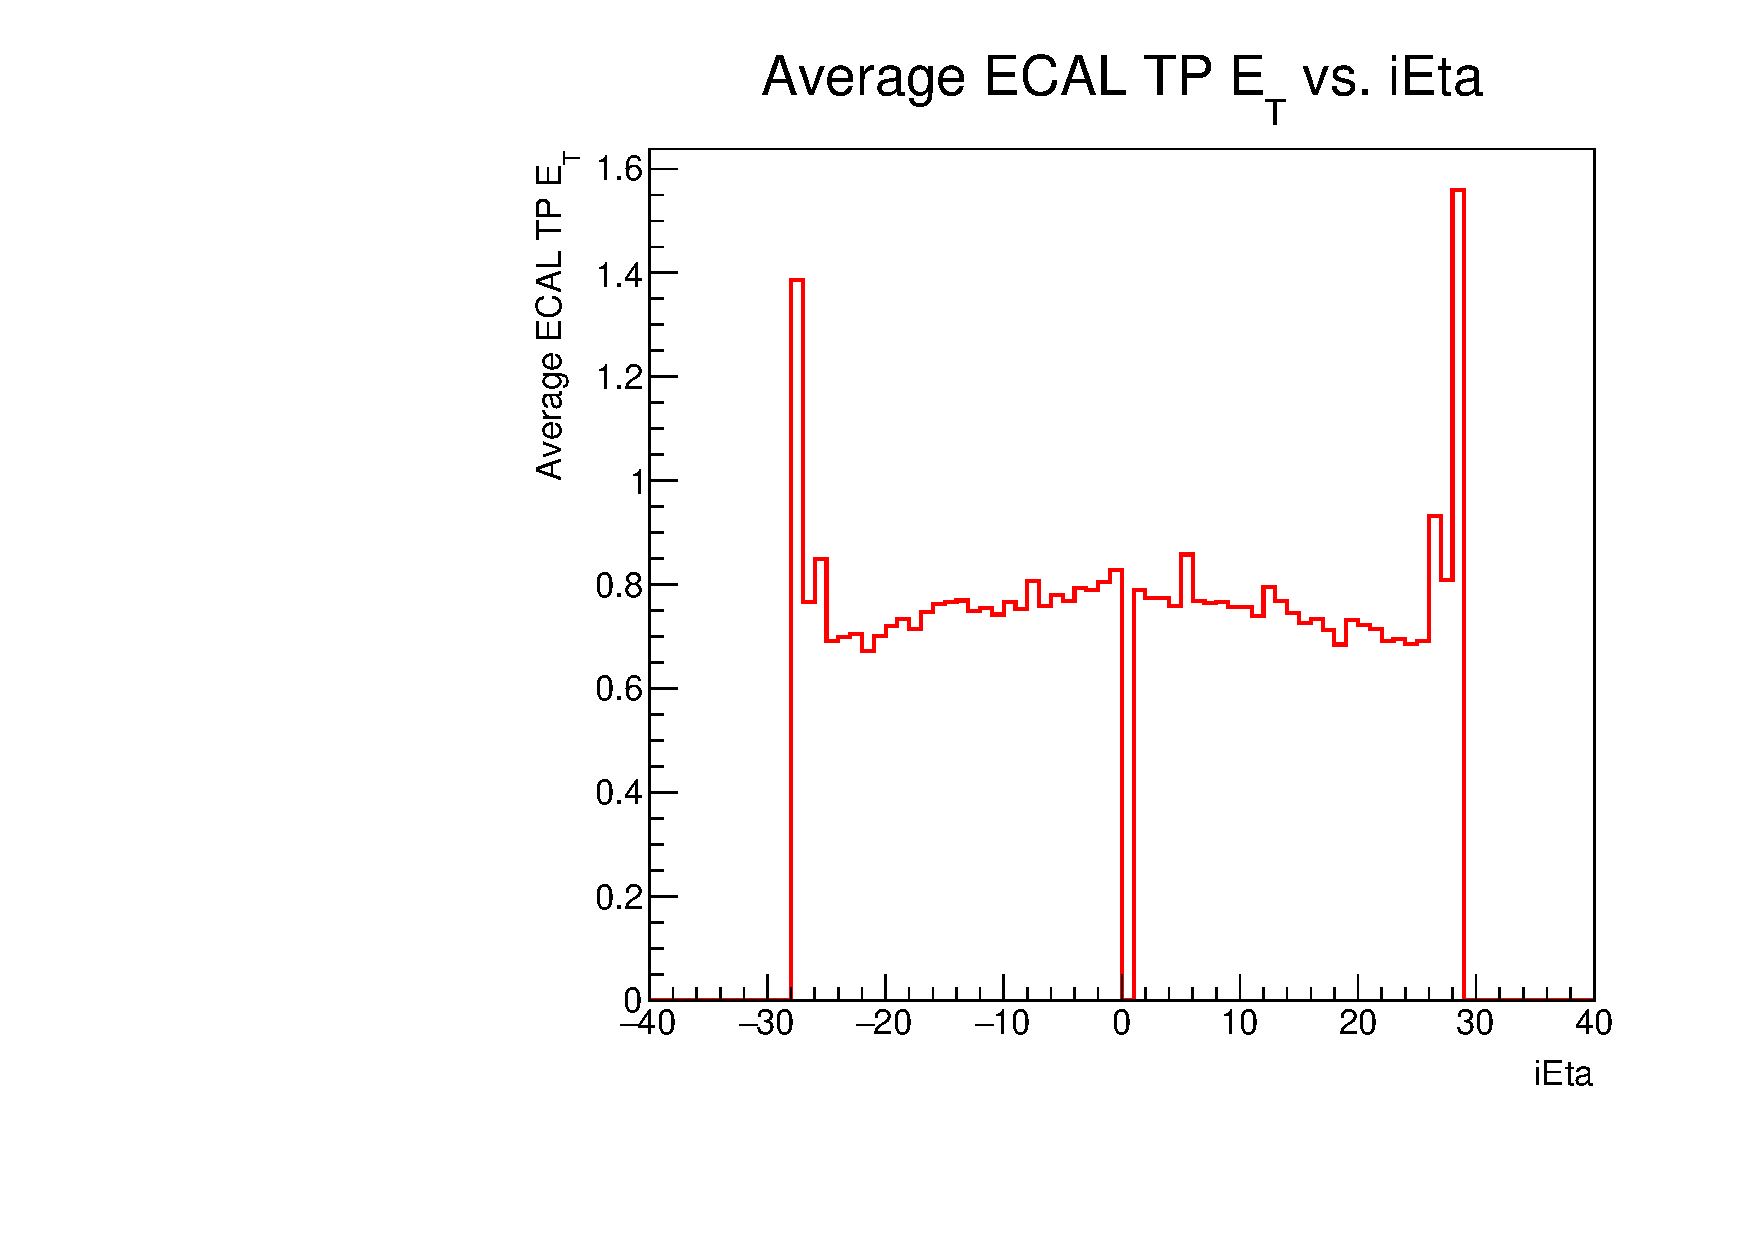
\includegraphics[width=110mm]{figures/MET_studies_v6/Plots/ECAL/ECALTPETEta.pdf}
\caption{The average TP $\ET$ (total TP $\ET$ in a bin divided by its occupancy) against iEta in the ECAL.}
\end{figure}

\begin{figure}[htbp]
\centering
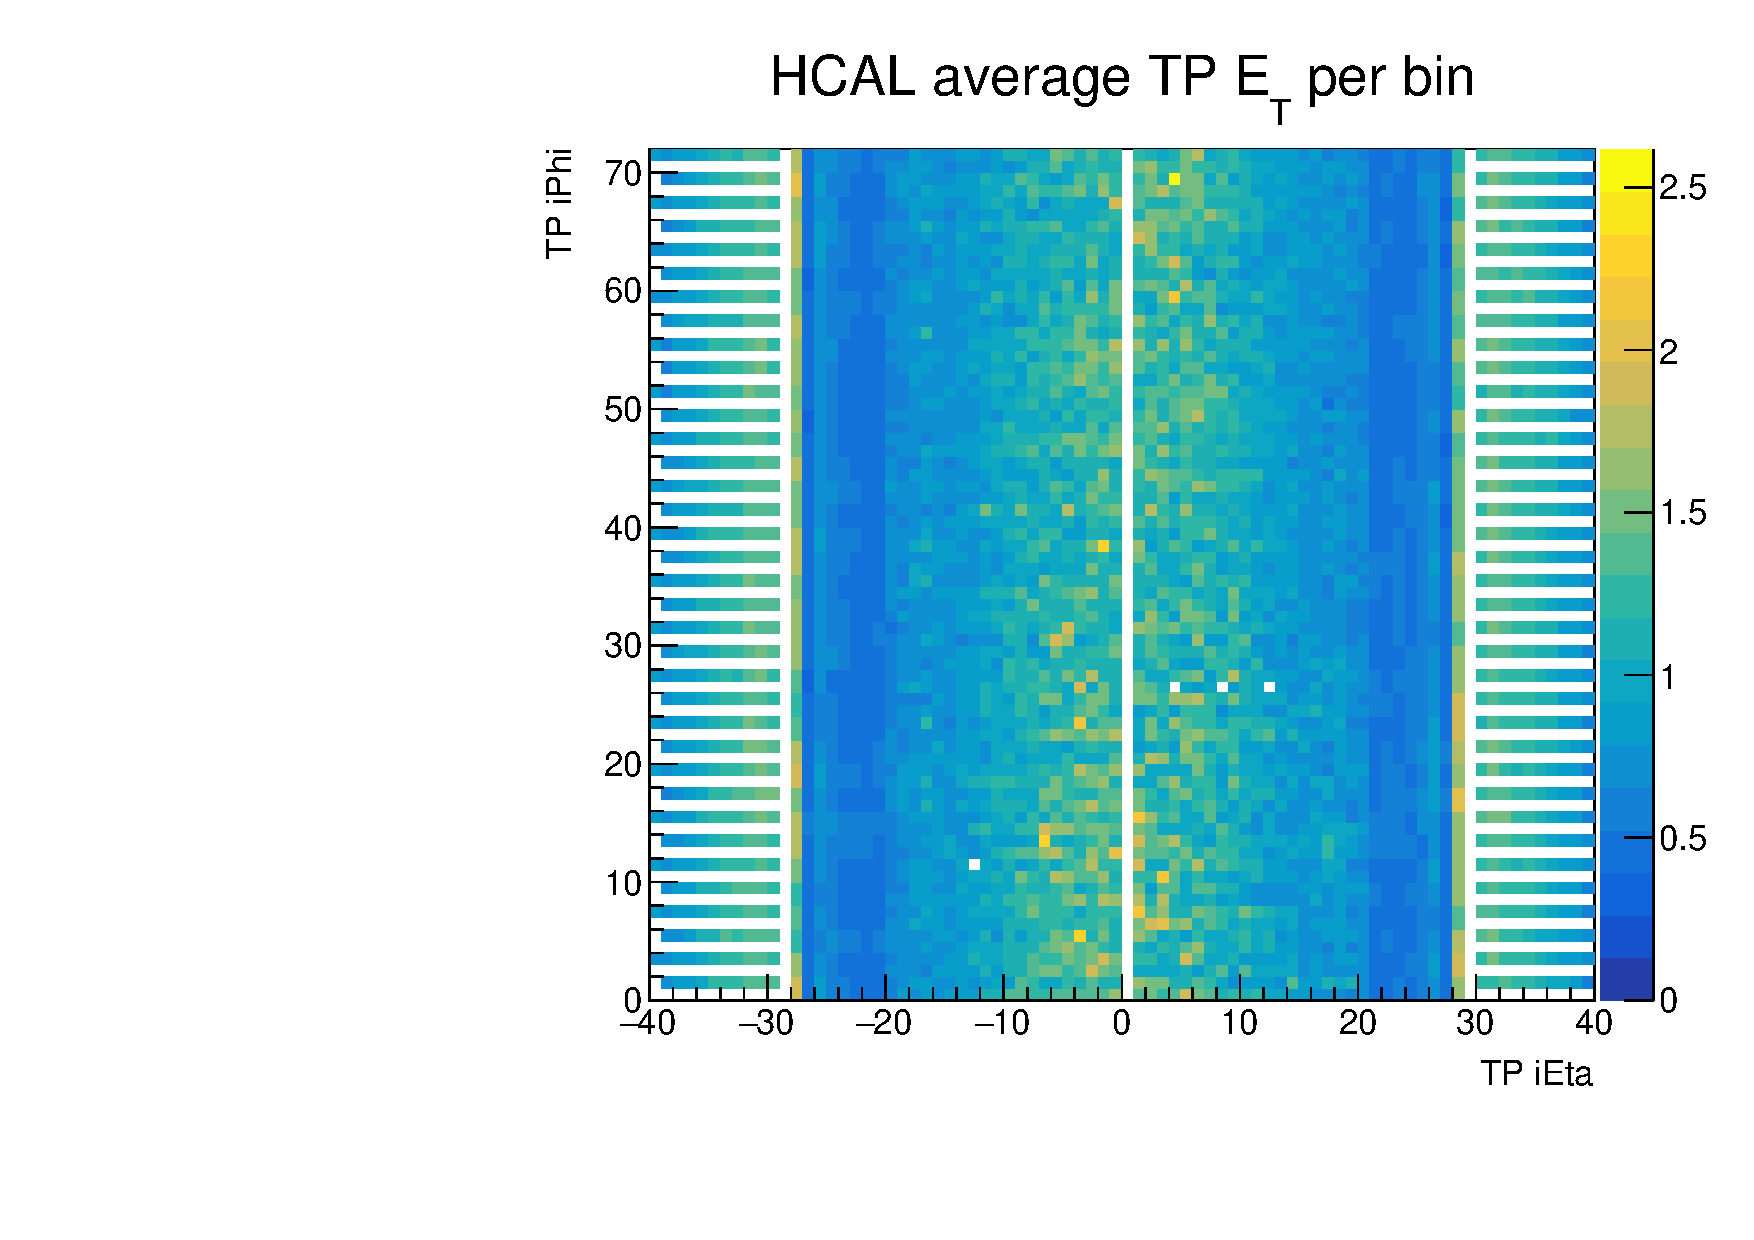
\includegraphics[width=110mm]{figures/MET_studies_v6/Plots/HCAL/HCALavgTPETEtaPhi.pdf}
\caption{The average TP $\ET$ against iEta and iPhi in the HCAL.}
\end{figure}

\begin{figure}[htbp]
\centering
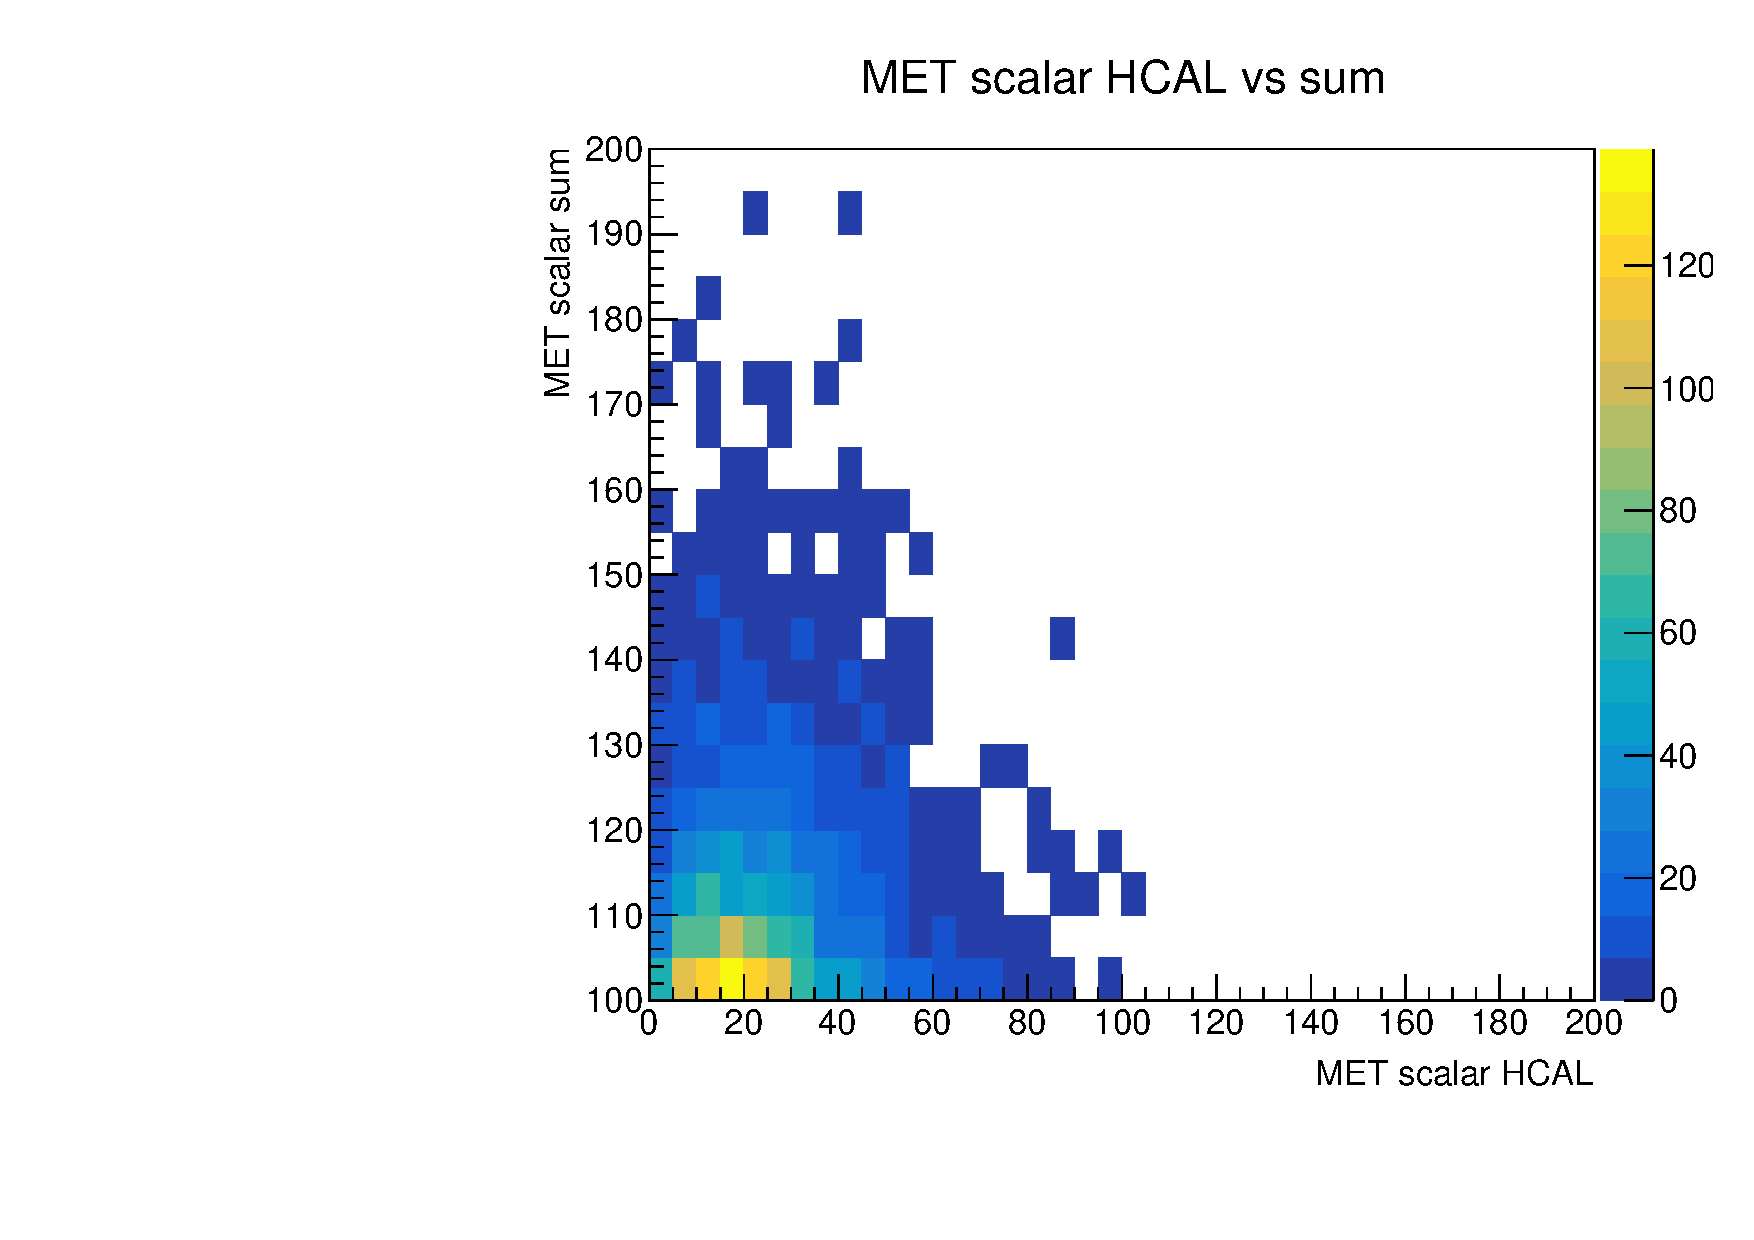
\includegraphics[width=110mm]{figures/MET_studies_v6/Plots/MetScalHcaltotal.pdf}
\caption{The \etmiss scalar in the HCAL vs the tower (sum).}
\end{figure}

Some of the plots have been shown in TPG meetings, one of which is here: \sloppy\url{https://indico.cern.ch/event/698504/contributions/2864568/attachments/1587832/2511546/2018_01_23_L1T_MET_TPs_Esh.pdf}.



% WILL BE USEFUL LATER ON
\if
The first thing I needed to do was clone the \textbf{cms-l1t-analysis} repo (\url{https://github.com/cms-l1t-offline/cms-l1t-analysis}) on Soolin. This contains code to make various plots and conduct studies about objects in the Level-1 Trigger. Once I've cloned the repo, I need to set everything up for the first time with

\begin{lstlisting}[belowskip=-0.7cm, language=sh, numbers=none]
cd <path>/cms-l1t-analysis
source bin/env.sh
make setup
\end{lstlisting}

and then to start a session in the future, I can use

\begin{lstlisting}[belowskip=-0.7cm, language=sh, numbers=none]
source bin/env.sh
voms-proxy-init --voms cms --valid 168:00 # if my grid cert. proxy has expired
\end{lstlisting}

The rest of the README is only really relevant if I'm contributing to the development of the repo. On the master branch, I need to make a config to store the dataset information I want (see \textbf{config/offline\_met\_studies.yaml} for a template) and an analyzer to take in the config and create the plots I want (see \textbf{cmsl1t/analyzers/offline\_met\_analyzer.py} for a template). This should be everything I need to add to make the MET plots.

In the config, when specifying the root file(s) I want to run over, I can use xrootd to check the leaves and trees so I know what to reference. I'll need a valid grid certificate proxy to be able to access the service. In a \ROOT session, I can open the file as normal, e.g.,

\begin{lstlisting}[belowskip=-0.7cm, language=C++, numbers=none]
TFile *f = TFile::Open("root://eoscms.cern.ch//eos/cms/store/group/dpg_trigger/comm_trigger/L1Trigger/safarzad/2017/ZeroBias/Collision2017-noRECO-l1t-integration-96p20/ZeroBias/crab_Collision2017-noRECO-l1t-integration-96p20__ZeroBias_Run2017C/170726_094745/0000/L1Ntuple_1.root")
\end{lstlisting}

then I can just open a TBrowser. The root file will be located in \textbf{\ROOT files/}, as seen in the TBrowser window. Note that whilst I can use wildcarding in the config, for obvious reasons I have to specify the exact path when using xrootd.

\fi



\section{Rate vs PU in JetMET for DPS note}

Every year, a DPS (Detector Performance Summary) note is produced for each object group in the trigger (muons, jetMET, etc.). For the 2017 performance for JetMET, Aaron and I have been working on the plots to showcase how the trigger has performed for those objects. I've been asked to make the rate vs PU plots with and without the MET PUS (pileup subtraction). Olivier and Chiara (VBF, taus) have code to calculate the rates at \url{https://github.com/camendola/RateStudies}, so I followed the README and made the relevant tweaks for JetMET.

The first thing was to get the PU and lumi section for a few runs, which I could do with \texttt{brilcalc}. I had to install and initialise it (on lxplus) with

\begin{lstlisting}[belowskip=-0.7cm, language=sh, numbers=none]
export PATH=$HOME/.local/bin:/afs/cern.ch/cms/lumi/brilconda-1.1.7/bin:$PATH # Needed each time to initialise
pip install --install-option="--prefix=$HOME/.local" brilws
\end{lstlisting}

and then I could run it with

\begin{lstlisting}[belowskip=-0.7cm, language=sh, numbers=none]
brilcalc lumi -r <run_no> --byls
\end{lstlisting}

I should get a table printed to the screen with the relevant info. But I need good lumi sections to work with. If I head to \url{https://cmswbm.cern.ch/cmsdb/servlet/RunSummary} and enter the run number, then submit and click on the run number hyperlink, it gives me a summary. Then, if I go to Other services $\rightarrow$ Lumi Sections, I'll get a green and red grid. By looking in the Physics column, it starts off red and then becomes green. I can take the time at which the column goes green, and then copy the entries from the table I got from running \texttt{brilcalc} that are after that time, which have the label "STABLE BEAM". Or I can append the brilcalc command with \texttt{> <name>.txt} and remove the entries I don't need from the file created. Then, I need to format the file so the columns are in the order of fill, run, lumi section, avg. PU. Visual Studio Code shortcuts can come in very handy if I want to use a GUI.

I then had to add a list of the ntutples I wanted to run over into a text file, and write a command in \textbf{scripts/EvalRatePU.sh} to execute it. The repo wasn't configured to run on Condor, so I had to add support for it in order to run at lxplus.

\textbf{Note: I couldn't get MET support added in time for the approval of the plots, so they never ended up in the note.}


